\documentclass[10pt,letterpaper]{article}
\usepackage{tikz}
\usetikzlibrary{bayesnet}

\begin{document}

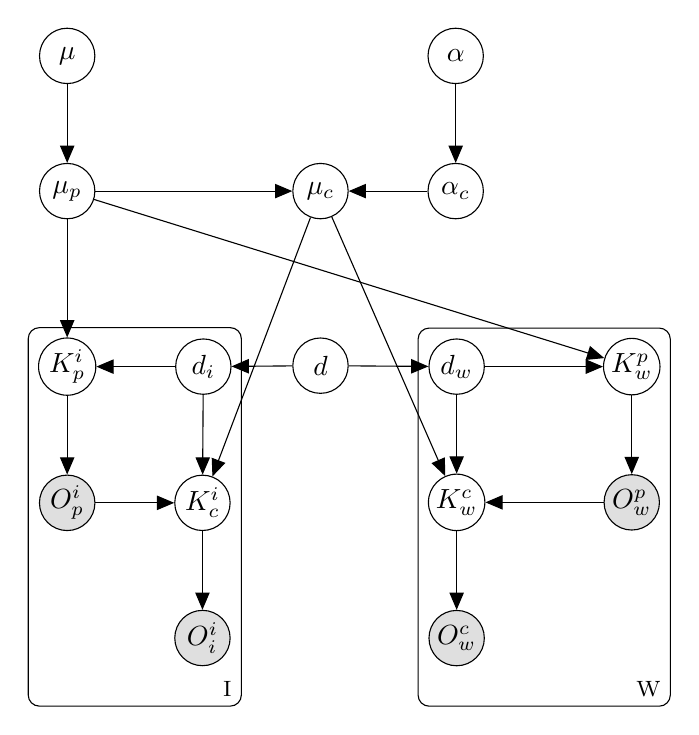
\begin{tikzpicture}[x=1cm,y=1cm]
  
   % Nodes
  \node[latent, ] (mu) {$\mu$};
  \node[latent, below = of mu] (mu_p) {$\mu_{p}$};
  \node[latent, right= 2.5 of mu_p] (mu_c) {$\mu_{c}$};

  \node[latent, right = of mu_c] (alpha_c) {$\alpha_{c}$};
  \node[latent, above = of alpha_c] (alpha) {$\alpha$};

  \node[latent, below = 1.5 of mu_p] (K_p_i) {$K_{p}^{i}$};
  \node[obs, below = of K_p_i] (O_p_i) {$O_{p}^{i}$};

  \node[latent, right = of O_p_i] (K_c_i) {$K_{c}^{i}$};
  \node[obs, below = of K_c_i] (O_c_i) {$O_{i}^{i}$};

  \node[latent, right = of K_p_i] (d_i) {$d_{i}$};
  \node[latent, right = 2.5 of d_i] (d_w) {$d_{w}$};



  \node[latent, right = 1.5 of d_w] (K_p_w) {$K^{p}_{w}$};
  \node[obs, below = of K_p_w] (O_p_w) {$O^{p}_{w}$};

  \node[latent, left = 1.5 of O_p_w] (K_c_w) {$K^{c}_{w}$};
  \node[obs, below = of K_c_w] (O_c_w) {$O^{c}_{w}$};

  \node[latent, below = 1.5 of mu_c] (d) {$d$};


  % Edges
  \edge{mu}{mu_p};
  \edge{mu_p}{mu_c};
  \edge{mu_c}{K_c_i};
  \edge{mu_p}{K_p_i};

  \edge{d}{d_w}
  \edge{d}{d_i}

  \edge{d_w}{K_c_w}
  \edge{d_i}{K_c_i}

  \edge{d_w}{K_p_w}
  \edge{d_i}{K_p_i}

  \edge{K_c_i}{O_c_i};
  \edge{mu_c}{K_c_w};
  \edge{K_c_w}{O_c_w};

  \edge{K_p_i}{O_p_i};
  \edge{mu_p}{K_p_w};
  \edge{K_p_w}{O_p_w};

  \edge{alpha}{alpha_c}
  \edge{alpha_c}{mu_c}

  \edge{O_p_w}{K_c_w}
  \edge{O_p_i}{K_c_i}

  % Plates
  \plate {plate_i} {(K_c_i)(O_c_i)(d_i)(K_p_i)(O_p_i)} {I};
  \plate {plate_w} {(K_c_w)(O_c_w)(d_w)(K_p_w)(O_p_w)} {W};  
\end{tikzpicture}

\end{document}